\chapter{Linear Systems with N Degrees of Freedom}
\section{Lumped parameter systems}
\subsection{1 Degree of Freedom}
	The idea of \de{lumped system} is to concentrate the \textbf{parameters} of the system, in particular:
	\begin{itemize}
		\item the \de{springs elements} where mostly of the elastic energy is stored (conservation of energy) and is assumed to be mass-less. Considering the \textbf{SCHEMATIC} of such element, we see that it's graphical representation present two connecting point that model the position on where the two ends of the springs are attached; those ends are subjected to forces $F_1,F_2$ and considering is center of gravity $G$ we have that, for Newton
		\[ \sum_i F_i = \cancelto 0{m \ddot x_G} \qquad \Rightarrow \qquad F_1 = F_2 = F\]
		We have so proven that such lumped spring elements doesn't permit load unbalance to their ends; regarding the behaviour of the system, is we assume that's the spring it's linear we can consider the force as linearly proportional to displacement, hence
		\begin{equation}
			F = k \big(x_2-x_1\big)
		\end{equation}
		where $k$ is the \de{stiffness} of the spring. When $x_2 -x_1 = 0$ we have that the spring absorbs no force;
		
		\item the \de{damper elements} describing the dissipative forces related to velocity; this element is still mass-less. Considering it's \textbf{SCHEMATIC}, the Newton equations determines
		\[ \cancelto0{m\ddot x_G} = F_2 - F_1 \qquad \Rightarrow \qquad F_2 = F_1 = F \]
		hence, as for the spring, such element isn't allowed to have different forces transmitted through it's ends. If we consider a \textbf{linear dumper} model the generated force $F$ can be regarded as
		\begin{equation}
			F = c \big(\dot x_2 - \dot x_1\big)
		\end{equation}
		where $c$ is the \de{viscous dumping} coefficient of the element;
		
		\item the \de{lumped mass} where all the mass of the system is concentrated and so contains the kinetic energy of the signal. Given $x$ the center of the mass of weight $m$, using Newton's law we have that
		\begin{equation}
			F = m \ddot x
		\end{equation}		
	\end{itemize}
	\textbf{AGGIUNGERE LE FIGURE}
	
	Real system aren't linear, however we can use the Taylor's series truncated to the first order to model every system as linear (within a certain range).
	
	\paragraph{Damped } Considering the system in \textbf{FIGURE} (FARE LA FIGURA) where the mass $m$ is subjected to it's body-weight force $mg$ (pointing downward) and an external force $f(t)$; setting to $y=0$ the coordinate were the elastic force is equal to zero, we can rewrite it's equation of motion by disassembling the components and considering the forces that they generates:
	\begin{align*}
		m \ddot y & = F_{spring} + F_{dumper} + F_{weigth} + f(t) \\
		& = - k y - c \dot y - mg + f(t)
	\end{align*}
	Such equation has a static solution, in fact if we consider $y_{st} = k\in \mathds R$ (hence $\dot y = \ddot y = 0$) we have that
	\[ 0 = -ky - mg \qquad \Rightarrow \qquad y_{st} = - \frac{mg}{k} \]
	Considering now the scale $x$ whose zero is for $y = - mg/k$ (the static solution of the differential equation), we have the substitution $x = y - y_{st}$ that determines the differential equation
	\begin{equation} \label{eq:lin1:temp1}
	\begin{aligned}
		m\big(\ddot x + \cancel{\ddot y_{st}}\big) & = - k (x+ y_{st}\big) - c \big(\dot x + \cancel{\dot y_{st}}\big) - mg + f(t) \\
		m\ddot x & = - k x - \cancel{(-mg)} - c\dot x -\cancel{ mg }+ f(t) \\
		m\ddot x + c\dot x + k x& = f(t)
	\end{aligned} 
	\end{equation}
	In this equation the first term $m\ddot x + c\dot x + kx$ represent the \de{logic of the system}, while on the right hand side $f(t)$ we have the \de{external action}, the input of the system.
	
	\subsubsection{Properties}
		Equation \ref{eq:lin1:temp1} represent an \textbf{ordinary linear differential equation} in the spatial dimension $x(t)$ with \textbf{constant coefficients} for the differential terms. In the particular case presented, having a non-zero term on the right-hand side we have that the differential equation is \textbf{non-homogeneous}.
		
	\subsubsection{General method for solving ordinary linear differential equations with constant coefficients}
		
		Given the linear ordinary differential equation with constant coefficient
		\begin{equation}
			a_n \frac{d^ny}{dt^n} + a_{n-1} \frac{d^{n-1}y}{dt^{n-1}} + \dots + a_0 y = b_m \frac{d^mu}{dt^m} + b_{m-1} \frac{d^{m-1}u}{dt^{m-1}} + \dots + b_0 u
		\end{equation}
		where $u$ represent the input of a system and $y$ it's output. Such system requires to known all the past history of the input to build the output, however considering it's states $x$. In order to find the solution we have to consider the following hypothesis:
		\begin{align*}
			i)& \qquad u(t) = 0 \qquad \textrm{for } t < 0 \\
			ii)& \qquad u(t) \textrm{is piecewise continuous} \\
			iii) & \qquad \textrm{states of the systems are known for } t = 0
		\end{align*}
		where the $n$ states $x_i$ are regarded as the output $y$ and all it's derivative up to order $n-1$, hence
		\[ x_1 = y(0) , \ x_2 = \dot y(0), \ \dots, \ x_n = y^{(n-1)}(0) \]
		If all this conditions are satisfied we can fined the solution $y(t)$ of the system as
		\begin{equation}
			y(t) = y_{homogeneous}(t) + y_{particular}(t)
		\end{equation}
	
		\paragraph{Solution of the homogeneous} The solution of the homogeneous is obtained by neglecting the input (right-hand side of the differential equation) and so considering only
		\[ a_n \frac{d^ny}{dt^n} + a_{n-1} \frac{d^{n-1}y}{dt^{n-1}} + \dots + a_0 y = 0 \]
		If we now consider each differentiation as a polynomial in a complex variable $\lambda \in \mathds C$ we have that
		\[ p(\lambda) = a_n \lambda^n + a_{n-1} \lambda^{n-1} + \dots + a_0 \lambda^0 = 0 \]
		The polynomial $p(\lambda)$ has $n$ roots that each can have a multiplicity $\mu_i$; associated to each root we have an associated homogeneous solution described as
		\begin{align*}
			y_{h,1} &= c_{11} e^{\lambda_1 t} + c_{12} t e^{\lambda_1 t} + \dots + c_{1\mu_1} t^{\mu_1-1} e^{\lambda_1 t} \\
			y_{h,2} &= c_{21} e^{\lambda_2 t} + c_{22} t e^{\lambda_2 t} + \dots + c_{2\mu_2} t^{\mu_2-1} e^{\lambda_2 t}
		\end{align*}
		hence in general for $N$ different roots we have
		\begin{equation}
			y_h(t) = \sum_{i=1}^{N} \sum_{j=1}^{\mu_i} c_{ij} t^{j-1} e^{\lambda_i t}
		\end{equation}
		
		\paragraph{Particular solution} To determine the solution it's necessary to find a function $y$ that satisfy the whole differential equation.
	
	\subsubsection{Laplace transform approach}
		Solution of linear ordinary differential equation can be obtained considering the \textbf{Laplace transform}
		\[ \laplace{f(t)} = F(s) := \int_0^\infty f(t) e^{-st}\, dt \qquad s\in \mathds C \]
		that transform differential equation in $t$ into algebraic equations in $s$, in fact it's proven that
		\[ \laplace{ f^{(n)}} = s^n F(s) - \sum_{i=0}^{n-1} s^{n-i-1}f^{(i)}(0) \]
		The idea is so to the find the solution in the domain of $s$ and then find the solution in time by using the inverse Laplace transform
		\begin{equation}
			f(t) = \antilaplace{F(s)} : = \frac 1{2\pi j} \int_{\alpha - j\infty}^{\alpha + j\infty} F(s) e^{st}\, ds \qquad \textrm{with } j = \sqrt{-1}
		\end{equation}
		This transformation is very useful due to the linearity property of $\mathscr L$, in fact
		\[ \laplace{a\, f(t) + b \,g(t)} = a \laplace{f(t)} + b \laplace{g(t)} \qquad \forall a,b \in \mathds C \]
		
		Using techniques in time we seen that in such domain the output of the system is the combination of terms in the form $t^n e^{at}$ whose transform is
		\begin{equation} \label{eq:lin:inverseexponential}
			\laplace{t^n e^{at}} = \frac{n!}{(s-a)^{n+1}} \qquad \forall n \in \mathds N,a\in \mathds C
		\end{equation}
		Applying this rule we can determine such common examples of Laplace transform as
		\begin{align*}
			\laplace{1(t)} & = \frac 1 s && a = n = 0 \\
			\laplace{\sin(\omega t)} = \laplace{\frac{e^{j\omega t} - e^{-j\omega t}}{2j}} & = \frac{\omega}{s^2 + \omega^2}&& n = 0, a = \pm j\omega
		\end{align*}	
		
		\paragraph{Application of the Laplace transform} Considering the differential equation \ref{eq:lin1:temp1} (page \pageref{eq:lin1:temp1}) defined as $m\ddot x + c\dot x + kx = f(t)$, we can find the solution in the $s$ domain applying the Laplace transform on such equation, determining:
		\begin{align*}
			m\big(s^2 X(s) - s x(0) - \dot x(s)\big) + c \big(sX(s) - x(0)\big) + kX(s) & = F(s) \\
			\big(ms^2 + cs - k\big)X(s) & = msx(0) + m\dot x(0) + cx(0) + F(s)
		\end{align*}
		We have so a polynomial problem in $s$ that can be solved determining
		\[ X(s) = \underbrace{\frac{msx_0+ m\dot x_0 + cx_0}{ms^2 + cs + k}}_\textrm{homogeneous sol.} + \underbrace{\frac{1}{ms^2 + cs + k}F(s)}_\textrm{particular sol.} \]
		The first term is usually called \textbf{free response} while the second is the \textbf{forced response}; the term $\frac{1}{ms^2 + cs + k} $ represent the \textbf{transfer function} of the system. From this expression we define the \de{natural angular frequency} $\omega_n$ and the \de{damping ratio} $\zeta$ defined as
		\begin{equation}
			\omega_n = \sqrt{ \frac k m} \hspace{2cm} \zeta =\frac{c}{c_c} = \frac{c}{2\sqrt{km}} = \frac{c}{2c \omega_n}
		\end{equation}
		This parameters allows to rewrite the response of the system as
		\begin{equation} \label{eq:lin1:temp2}
			X(s) = \frac{x_0s + \dot x_0 + 2 \zeta \omega_n x_0}{s^2 + 2 \zeta\omega_ns + \omega_n^2} + \frac{1/m}{s^2 + 2 \zeta \omega_n s + \omega_n^2} F(s)
		\end{equation}
		
		In general the solution in the Laplace domain can be described as a sum of the homogeneous solution and the particular one as rational polynomial in the form
		\[ X(s) = \frac{A(s)}{B(s)} + \frac{N(s)}{D(s)} U(s) \]
		We refer to the roots of the nominators $A(s),N(s)$ as \textbf{zeros} while the one of the denominators $B(s),D(s)$ are the \textbf{poles}.
	
		Returning to the example, the poles $p_i$ of the homogeneous term in equation \ref{eq:lin1:temp2} can be simply calculates as
		\[ p_{1,2} = - \zeta \omega_n \pm \sqrt{\zeta^2\omega_n^2 - \omega_n^2} = -\zeta \omega_n \pm \omega_n \sqrt{\zeta^2 - 1} \]
		Depending on the value of the damping ratio $\zeta$ the poles can be real ($\zeta > 1$) or complex conjugated (for $\zeta < 1$). In particular the cases are
		\begin{itemize}
			\item if $\zeta = 0$ we have the poles in $p_{1,2} = \pm j\omega_n$ that are purely imaginary and each pole has a multiplicity $\mu = 1$;
			\item if $0 < \zeta< 1$ the poles are $p_{1,2} = - \zeta \omega_n \pm j\omega_n \sqrt{1-\zeta^2}= -\zeta \omega_n \pm j\omega_d$ and so are complex conjugated. The magnitude of such complex root is
			\[ |p_{1,2}| = \sqrt{\zeta^2 \omega_n^2 + \omega_n^2(1-\zeta^2)} = \omega_n \]
			\item if $\zeta = 1$ we have a double root (multiplicity $\mu = 2$) in $p_{1,2} = - \omega_n$;
			\item if $\zeta> 1$ the poles are purely real $p_{1,2} = -\zeta \omega_n \pm \omega_n \sqrt{\zeta^2-1}$ and their multiplicity is unitary ($\mu = 1$).
		\end{itemize}
		
		\paragraph{Time response of the homogeneous} Considering the homogeneous term, assuming the initial state as zeros ($x_0 = 0$) for simplicity we have
		\[ X_h(s) = \frac{ \dot x_0}{s^2 + 2 j\omega_ns + \omega_n^2} \]
		Applying the partial fraction decomposition we can obtain a transfer function in the form (where we consider that all poles have multiplicity $\mu =1$, so the case $\zeta = 1$ cannot be described by this expression):
		\[ X_h(s) = \frac{R_{1h}}{s-p_1} + \frac{R_{2h}}{s-p_2} \]
		We can compute the residuals as
		\begin{align*}
			R_{1h} & = \left.\left[ (s-p_1) X_h(s)\right] \right|_{s=p_1} = \frac{\dot x_0}{p_1-p_2} \\
			R_{2h} & = \left.\left[ (s-p_2) X_h(s)\right] \right|_{s=p_2} = \frac{\dot x_0}{p_2-p_1} 		
		\end{align*}
		Considering the result of equation \ref{eq:lin:inverseexponential} we can consider the partial fraction decomposition with parameters $n=0$ and $a = p_1,p_2$. In particular considering the linearity we have that
		\[ x_h(t) = \antilaplace{X(s)} = R_{1h} t^0 e^{p_1t} + R_{2h} t^0 e^{p_2t} = R_{1h} e^{p_1t} + R_{2h} e^{p_2t}  \]
		Depending on the \textit{type} of the poles (real or imaginary), the general behaviour of the system might differs and we have to use mathematical complex equation to determine the final expression in time. Furthermore if $0 < \zeta < 1$ we have complex conjugated poles in the form $p_{1,2} = -\zeta \omega_n \pm j\omega_d$ (with $\omega_d = \omega_n\sqrt{1-\zeta^2}$ the \textbf{\textit{damped natural frequency}}), hence the residuals becomes
			\[ R_{1h} = \frac{\dot x_0}{p_1-p_2} = \frac{\dot x_0}{2j \omega_d} \frac{-j}{-j} = - j \frac{\dot x_0}{2\omega_d}  \hspace{2cm} R_{2h} = j \frac{\dot x_0}{2\omega_d} \]
			Observing that the residual are also complex conjugated ($R_{2h} = R_{1h}^*$) as the poles, we can write the full solution of the homogeneous in the time domain as
			\begin{equation}
			\begin{aligned}
				x_h(t) & = R_{1h} e^{p_1t} + R_{2h} e^{p_2t} \\
				& = 2 \frac{\dot x_0}{2\omega_d} e^{-\zeta \omega_n t} \cos\left( -\frac \pi 2 + \omega_d t \right) = \frac{\dot x_0}{\omega_d} e^{-\zeta \omega_n t} \sin\left( \omega_d t \right)
			\end{aligned}
			\end{equation}
			This is a \textit{pseudo-periodic} function with period $T = \frac {2\pi }{\omega_d}$.
			
			
		\paragraph{Time response of the particular solution} Considering the particular solution that in the time domain is expressed as
		\[ X_p(s) = \frac{1/m}{s^2 + 2 \zeta \omega_n s + \omega_n^2} F(s) \]
		Considering the  input as a unit step function of amplitude $F_0$, we have that it's transform is determined by
		\[ F(s) = \laplace{ F_0 u(t)} = F_0 \frac 1 s \qquad \Rightarrow \quad X_p(s) = \frac{F_0}{m} \frac{1}{s^2 + 2\zeta\omega_ns + \omega_n^2} \frac 1 s \]
		The poles of the overall systems are so $p_{1,2} = -\zeta \omega_n \pm \omega_n \sqrt{\zeta^2 - 1}, p_3 = 0$, rewriting the particular solution with the related partial fraction decomposition
		\[ X_p(s) = \frac{F_0}m \frac{1}{(s-p_1)(s-p_2)} \frac 1 s = \frac{R_{1p}}{s-p_1} + \frac{R_{2p}}{s-p_2} + \frac{R_{3p}}{s} \]
		where the decomposition in made on the assumption of unitary multiplicity ($\mu_i = 1$ hence $\zeta \neq 1$). Computing
		\begin{align*}
			R_{1p} & = \left.\left[ (s-p_1) X_p(s)\right] \right|_{s=p_1} = \frac{F_0}{m} \frac{1}{(p_1-p_2)p_1} \hspace{1cm}
			R_{2p} = \left.\left[ (s-p_2) X_p(s)\right] \right|_{s=p_2} = \frac{F_0}{m} \frac{1}{(p_2-p_1)p_2} \\
			R_{3p} & = \left.\left[ s X_p(s)\right] \right|_{s=0} = \frac{F_0}{m} \frac{1}{p_1p_2} 
		\end{align*}
		The particular solution in the time domain is so obtained with the inverse Laplace transform
		\begin{align*}
			x_p(t) & = \antilaplace{ \frac{R_{1p}}{s - p_1} + \frac{R_{2p}}{s-p_2} + \frac{R_{3p}}{s} }  = R_{1p}e^{p_1t} + R_{2p}e^{p_2t} + R_{3p}e^{p_3t}
		\end{align*}
		In particular when we have $0 < \zeta < 1$ we have to complex conjugated poles $p_{1,2} = - \zeta \omega_n \pm j \omega_d$ (with $\omega_d = \omega_n \sqrt{1-\zeta^2}$) determines the residuals $R_{1p} = \frac{F_0}m \frac {1}{2j\omega_d} \frac{1}{-\zeta \omega_n + j\omega_d}$, $R_{2p} = \frac{F_0}m \frac {1}{-2j\omega_d} \frac{1}{-\zeta \omega_n - j\omega_d}$ and $R_{3p} = \frac{F_0}{m } \frac{1}{\omega_n^2} = \frac{F_0}{k}$; we so have that
		\begin{align*}
			x_p(t) &  = |R_{1p}| e^{ \Re{p_1} t } \cos\left( \Im{p_1} t + \arg\{R_{1p}\} \right) + R_{3p} e^{0t} \hspace{2cm} \textrm{with } \zeta \in (0,1 )\\ & 
			= \frac{F_0}{m} \frac{1}{\omega_n^2\sqrt{1-\zeta^2}} e^{ -\zeta \omega_n t } \cos\left( \omega_d t - \frac \pi 2  - \big(\pi-\theta\big) \right) + \frac{F_0}{k} \\
			& = \frac{F_0}{k} \frac{1}{\sqrt{1-\zeta^2}} e^{ -\zeta \omega_n t } \cos\left( \omega_d t +\theta - \frac 3 2 \pi \right) + \frac{F_0}{k} \\ 
			& = \frac{F_0}{k} \left( 1 - \frac{e^{-\zeta \omega_n t}}{\sqrt{1-\zeta^2}} \sin\left( \omega_d t + \theta \right) \right) u(t) \\ 
		\end{align*}
		
		\paragraph{Overall system response} Hypothesising as initial condition $x_0 = 0$ and $\dot x_0 \neq0$ with a damping $\zeta \in (0,1)$, then the overall response of the system in the Laplace domain can be decomposed in two parts: one associated to the transients (decaying exponential) and one relegated to the steady state response of the system:
		\begin{equation}
			X(s) = \underbrace{\frac{R_{1h}}{s - p_1} + \frac{R_{2h}}{s-p_2} + \frac{R_{1p}}{s - p_1} + \frac{R_{2p}}{s-p_2} }_\textrm{transient}+ \underbrace{\frac{R_{3p}}{s}}_\textrm{steady state}
		\end{equation}
		This relates to the following time response:
		\begin{equation}
		\begin{split}
			x(t) & = \Bigg[ \underbrace{\frac{\dot x_0}{\omega_d} e^{-\zeta \omega_n t} \sin\left( \omega_d t \right)}_\textrm{homogeneous} + \underbrace{\frac{F_0}{k} \left( 1 - \frac{e^{-\zeta \omega_n t}}{\sqrt{1-\zeta^2}} \sin\left( \omega_d t + \theta \right) \right)}_\textrm{particular}  \Bigg]u(t) \\
			& = \Bigg[ \underbrace{\frac{\dot x_0}{\omega_d} e^{-\zeta \omega_n t} \sin\left( \omega_d t \right) - \frac{F_0}{k}\frac{e^{-\zeta \omega_n t}}{\sqrt{1-\zeta^2}} \sin\left( \omega_d t + \theta \right) }_\textrm{transient} + \underbrace{\frac{F_0}{k}}_\textrm{steady state}  \Bigg]u(t) \\
		\end{split}
		\end{equation} 
	
	\subsection{Frequency response of a system}
		We can analyse systems also considering inputs $u(t)$ that are sinusoidal, hence in the form $M  \sin (\omega t)$ characterized by a transform
		\[ U(s) = M \frac{\omega}{s^2+ \omega^2} \]
		Considering that the output in the Laplace domain is in the form $Y(s) = \frac{A(s)}{B(s)} + \frac{N(s)}{D(s)} U(s)$ where $N(s)/D(s)= G(s)$ is the \textbf{transfer function} of the system. Assuming that the roots of both $B(s)$ and $D(s)$ are all \textit{stable} (meaning that doesn't have positive real part), we have the response that for a $2^{nd}$ order system can be regarded as
		\begin{align*}
			 Y(s) & = \frac{A(s)}{B(s)} +G(s) M \frac{\omega}{s^2 + \omega^2} \\ &   = \frac{A(s)}{(s-p_1)(s-p_2)} + \frac{N(s)}{(s-p_1)(s-p_2)} M \frac{\omega}{(s-j\omega)(s+j\omega)} \\ 
			 & = \frac{R_{1h}}{s - p_1} + \frac{R_{2h}}{s-p_2} + \frac{R_{1p}}{s - p_1} + \frac{R_{2p}}{s-p_2} + \frac{R_{3p}}{s-j\omega} + \frac{R_{4p}}{s+j\omega}
		\end{align*}
		By applying the reverse Laplace transform
		\[ y(t) = \underbrace{R_{1h} e^{p_1t} + R_{2h} e^{p_2t} + R_{1p} e^{p_1t} + R_{2p} e^{p_2t}}_\textrm{same time constant $\tau$ of decay} + R_{3p} e^{j\omega t} + R_{4p} e^{-j\omega t} \]
		Neglecting the transient we have that the resulting output is a linear combination of exponential in the form $ y(t) R_{3p} e^{j\omega t} + R_{4p} e^{-j\omega t}$; considering that $R_{4p} = R_{3p}^*$ we obtain that $y(t) = 2 |R_{3p}| e^{0 t} \cos(\omega t + \arg\{ R_{3p} \})$ (for $t\gg \tau$). We can compute the residuals as
		\[ R_{3p} = \left[ \cancel{(s-j\omega)} G(s) M \frac {\omega}{\cancel{(s-j\omega)}(s+j\omega)}  \right] \Bigg|_{s=j\omega} = \frac{G(j\omega) M}{2j} \hspace{2cm} R_{4p} = - \frac{G(-j\omega) M}{2j}  \]		
		This results in the following steady state response in the time domain representing the so called \de{frequency response function}:
		\begin{equation}
			y_{ss}(t) = 2 \frac M 2 |G(j\omega)| e^{0t} \cos\left( \omega t + \arg\{ G(j\omega) \} - \frac \pi 2\right) = M G(j\omega) \sin(\omega t + \varphi(j\omega))
		\end{equation}
		where $|G(j\omega)$ is the magnitude and $\varphi(j\omega)$ is the phase of the transfer function. Graphically a sinusoidal input is \textit{amplified} by a factor $G(j\omega)$ (that so depends on the pulsation $\omega$ of the input) and \textit{shifted} by a time $\frac{2\pi}{\varphi(j\omega)}$ (the peak of the output is \textit{on the right} respect to the input in order to have causal systems). The frequency response function, given the transfer function $G(s)$, is computed considering $s=j\omega$; as example if we have
		\[ G(s) = \frac 1 m \frac{1}{s^2 + 2 \zeta\omega_n s + \omega_n^2} \qquad \Rightarrow \qquad G(j\omega) = \frac 1 m \frac{1}{(j\omega)^2 + 2 \zeta \omega_n (j\omega) + \omega_n^2} = \frac{1/k}{1 - \left( \frac \omega {\omega_n} \right)^2 + 2 j \zeta \frac\omega{\omega_n} }  \]
		\[ \Rightarrow \qquad |G(j\omega)| = \frac{1/k} { \sqrt{ \left[ 1 - \left( \frac \omega {\omega_n} \right)^2  \right]^2 + 4 \zeta^2 \left(\frac \omega {\omega_n}\right)^2 }  }  \qquad \varphi(j\omega) = - \arctan\left( \frac{2 j \frac{\omega}{\omega_n}}{1 -\left( \frac \omega {\omega_n}\right)^2  } \right) \]
		Usually $|G(j\omega)|$ and $\varphi(j\omega)$ are represented in \textbf{Bode plots} \textbf{VEDERE APPUNTI}; defining the quality factor $Q$ as the magnitude at the maximum frequency $k |G(j\omega_{peak})|$ and so
		\[ Q = \frac{1}{2\zeta \sqrt{1-\zeta^2}} \qquad \xrightarrow{\zeta \textrm{ small}} \quad Q \approx \frac 1{2\zeta} \]
		Such approximation allows to experimentally determine the damping coefficient of the system; \textbf{VEDERE GRAFICO APPUNTI}
		
	
	\subsubsection{Convolution integral}
		Analysing systems in the Laplace domain we observed that the output $Y(s)$ is achieved by multiplying the transfer function $G(s)$ by the transform of the input $U(s)$ in case of zero initial conditions:
		\[ Y(s) = G(s) U(s) \]
		If we determine an input $u(t)$ characterized by the transform $U(s)$, what will we observe is that the output matches the transfer function: $Y(s) = G(s) 1 = G(s)$. Building the function
		\[ f(t,\tau) = \frac 1 \tau \Big[ u_s(t) - u_s(t-\tau) \Big] \]
		what we obtain is a rectangular pulse of amplitude $1/\tau$ and width $\tau$ (given $u_s(t)$ the unit step function); by pushing $\tau\rightarrow 0$, $f$ tends to the \textbf{Dirac pulse/delta} $\delta(t)$, a distribution characterized by being zero $\forall t \neq 0$ where it evaluates at $\infty$; such function is characterized by having $\int_{-\infty}^\infty \delta(t) \, dt = 1$ and has the important property $\int_{\infty}^{\infty} g(t) \delta(t)\, dt = g(0)$ for any function $g(t)$. To compute the transform of $f$ respect to $t$ we can use the linear property of the Laplace transform and we obtain
		\[ F(s,\tau) = \frac 1 \tau \frac 1 s - \frac 1 \tau \frac 1 s e^{-\tau s} = \frac 1{\tau s} \left( 1 -e^{-\tau s} \right) \qquad  \xrightarrow{\tau \rightarrow 0} \qquad \lim_{\tau \rightarrow 0} \frac{1-e^{-\tau s}}{\tau s} \]
		Using De L'Hopital rule what we obtain is that
		\[ F(s,\tau\rightarrow 0) = \lim_{\tau \rightarrow 0} \frac{s e^{-\tau s}}{s} = 1 \]
		
		By determining the output of the system subjected to a Dirac delta as input, the output that we obtain is the \de{impulse response} of the system $g(t) = y(t)$.
		
		\paragraph{Convolution theorem} Considering the convolution theorem stating that
		\begin{equation}
			\laplace{ \int_0^\infty f_1(\theta) f_2(t-\theta)\, d\theta} = F_1(s) F_2(s)
		\end{equation}
		by applying the inverse transformation we of course get the result
		$ \antilaplace{F_1(s) F_2(s)} = \int_0^\infty f_1(\theta) f_2(t-\theta)\, d\theta $.
		Knowing so that in the Laplace domain $Y(s) = G(s) U(s)$ we obtain that the output of the system in the time domain can be thought as the convolution between impulse response and input:
		\begin{equation}
			y(t) = \antilaplace{G(s) U(s)} = \int_0^\infty g(\theta)u(t-\theta) \, d\theta
		\end{equation}
		
		In practise stable systems are characterized by an impulse response that present a decay with a certain time constant $\tau$ (and so has a finite \textit{memory} on the history of the inputs) and by a computational point of view we don't have to compute the integral in the domain $(0,\infty)$, but $(0,t)$ is still ok.
		
		\paragraph{Alternative formulation} An alternative formulation of the convolution theorem is that the output can be regarded as
		\[ y(t) = \int_0^t u(\theta) g(\theta-t)\, d\theta \]
		In practise this means that the convolution operator $*$ is commutative, in the sense that
		\[ y(t) = (u*g)(t) = (g*u)(t) \]

\subsection{2 degrees of freedom}
	Considering now the case of a \de{two degrees of freedom} \textbf{system} as shown in \textbf{FIGURE DA FARE}, we can see that the dynamical equations of the system are
	\[ \begin{cases}
		m \ddot x_1 = - k_1 x_1 - c_1 \dot x_1 + k_2(x_2-x_1) + c_2(\dot x_2 - \dot x_1) + f_2 \\
		m_2 \ddot x_2 = k_2 (x_1-x_2) + c_2(\dot x_1 - \dot x_2) - k_3x_2 - c_3 \dot x_2 + f_2
	\end{cases} \]
	We can see that such system is linear regarding the positions $x_i$ and it's derivative, in fact it can be considered in a matrix notation as
	\begin{equation}
		\underbrace{ \matrix{m_1 & 0 \\ 0 & m_2}}_{\mat M} \vec{\ddot x_1 \\ \ddot x_2} + \underbrace{ \matrix{c_1+c_2 & - c_2 \\ - c_2 & c_2 + c_3}}_{\mat C} \vec{\dot x_1 \\ \dot x_2} + \underbrace{\matrix{k_1+k_2 & -k_2 \\ - k_2 & k_2+k_3}}_{\mat K} \vec{x_1 \\ x_2} = \vec{f_1 \\ f_2}
	\end{equation}
	where $\mat M, \mat C, \mat K$ are respectively the \textbf{mass}, \textbf{damping} and \textbf{stiffness} matrix. If we regard $\vett x = (x_1,x_2)$ and $\vett f = (f_1,f_2)$ the previous expression can be reduced to the form
	\begin{equation}
		\mat M \ddvett x + \mat C \dvett x + \mat K \vett x= \vett f
	\end{equation}
	
	As in the analysis of 1 degree of freedom systems, the solution can be obtained by applying the Laplace transform on this expression that's now a system of linear differential equations, resulting in:
	\[ \mat M\Big( s^2 \vett X(s) - s \vett x_0 - \dvett x_0 \Big) + \mat C \Big( s\vett X(s) - \vett x_0 \Big) + \mat K \vett x(s) = \vett F(s) \]
	that solved for the unknown $\vett X(s)$ determines the solution
	\begin{equation}
		\vett X(s) = \underbrace{\overbrace{\big(\mat M s^2 +\mat C s + \mat K\big)^{-1}}^{= \mat G(s)} \Big( (\mat M s + \mat C)\vett x_0 + \mat M \dvett x_0 \Big)}_\textrm{homogeneous solution} + \underbrace{\big(\mat M s^2 +\mat C s + \mat K\big)^{-1} \mat F(s) }_\textrm{particular sol.}
	\end{equation}
	In this representation $\mat G(s)$ is the \de{transfer function}, a $2\times 2$ matrix where each entry results in a rational polynomial in the complex variable $s$; such matrix can be regarded as the inverse of the matrix $\mat D$ defined as
	\[ \mat D = \mat M s^2 + \mat C s + \mat K = \matrix{d_{11} & d_{12} \\ d_{21} & d_{22}} = \matrix{ m_1 s^2 + (c_1+c_2)s + k_1 + k_2 & -c_2 s - k_2 \\ -c_s s - k_2 & m_2s^2 + (c_2+c_3)s + k_2 + k_3 } \]
	\[ \Rightarrow \qquad \mat G(s) = \mat D^{-1} = \frac 1{\det \mat D} \matrix{d_{22} & - d_{12} \\ - d_{21} & d_{11} } = \matrix{ G_{11}(s) & G_{12}(s) \\ G_{21}(s) & G_{22}(s) }   \]
	
	\paragraph{Particular solution} \textbf{DA VEDERE}
	
	\paragraph{Homogeneous solution} Considering now only the homogeneous term of the solution and assuming as initial states $\vett x_0 = (x_{10},0)$ and $\dvett x_0 =(0,0)$, what we obtain is
	\begin{align*}
		X_{hom}(s) & = \matrix{ G_{11}(s) & G_{12}(s) \\ G_{21}(s) & G_{22}(s) }  \matrix{ m_1 s + c_1 & 0 \\ 0 & m_2 s + c_3 } \vec{x_{10} \\ 0} \\ & = \vec{G_{11}(s) (m_1 s- c_1) x_{10} \\ G_{21}(s) (m_1s + c_3) x_{10} } = \vec{X_{h1}(s) \\ X_{h2}(s) }
	\end{align*}
	We can so compute separately the two components $X_{h1},X_{h2}$ of the solution. Knowing that the entry $G_{11}$ is expressed as $\frac{d_{22}}{d_{11}d_{22} - d_{12}d_{21}}$, by applying all the substitutions we obtain a rational polynomial of degree 4:
	\[ X_{h1}(s) = \frac{(m_1s + c_1) (m_2 s^2 + c_3 s + k_2 + k_3) x_{10}}{ (m_1 s^2 + c_1 s + k_1 + k_2)(m_2s^2 + c_3s + k_2+k_3) - k_2^2 } \]
	Such function has 4 roots $p_1,p_2,p_3,p_4$ of the denominator that can both be real or complex conjugated; assuming that such values are all distinct (meaning that the multiplicity of all poles is unitary) the resulting partial fraction decomposition is
	\[ X_{h1}(s) = \underbrace{\frac{R_{11}}{s-p_1} + \frac{R_{12}}{s-p_2}}_{X_{11}(s) \mapsto x_{11}(t) } + \underbrace{\frac{R_{13}}{s-p_3} + \frac{R_{14}}{s-p_4}}_{X_{13}(s)\mapsto x_{13}(t)} \]
	where usually the underlined terms are considered together because in for \textbf{RIVEDERE DEFINIZIONE} critical the poles are complex conjugated and their combined time response results in an exponentially decaying sinusoidal signal. Similarly we can compute the response of the second component $X_{h2}(s)$ of the solution reaching the partial fraction expansion
	\[ X_{h2}(s) = \underbrace{\frac{R_{21}}{s-p_1} + \frac{R_{22}}{s-p_2}}_{X_{21}(s) \mapsto x_{21}(t) } + \underbrace{\frac{R_{23}}{s-p_3} + \frac{R_{24}}{s-p_4}}_{X_{23}(s)\mapsto x_{23}(t)} \]
	This means that the homogeneous response (considering the preliminary assumption formulated) is in the form
	\[ X_{hom}(s) = \vec{R_{11} \\ R_{21} } e^{p_1 t} + \vec{R_{12} \\ R_{22} } e^{p_2 t} + \vec{R_{13} \\ R_{23} } e^{p_3 t} + \vec{R_{14} \\ R_{24} } e^{p_4 t} \]
	Assuming that the pairs of poles $p_1,p_2$ and $p_3,p_4$ are complex conjugated (as well as their residuals), the inversion of such transfer function is a linear combination of 2 oscillating exponentials:
	\begin{align*}
		x_{h1}(t) = x_{11}(t) + x_{13}(t) \qquad \textrm{where} \quad & x_{11}(t) = 2 |R_{11}| e^{\Re{p_1} t}\cos\big(\Im{p_1} t +\angle{R_{11}}\big) \\
		& x_{13}(t) = 2 |R_{13}| e^{\Re{p_3} t}\cos\big(\Im{p_3} t +\angle{R_{13}}\big)
	\end{align*}
	
	\begin{figure}[bht]
		\centering
		\begin{subfigure}{0.48\linewidth}
			\centering 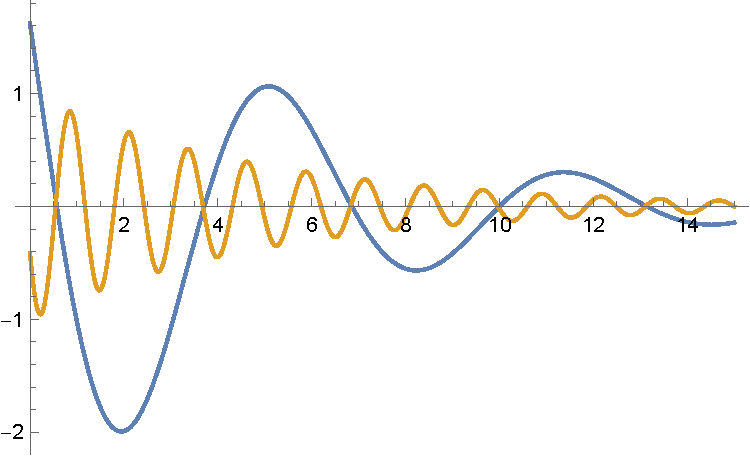
\includegraphics[width=\linewidth]{2dof-a} \caption{}
		\end{subfigure}
		\begin{subfigure}{0.48\linewidth}
			\centering 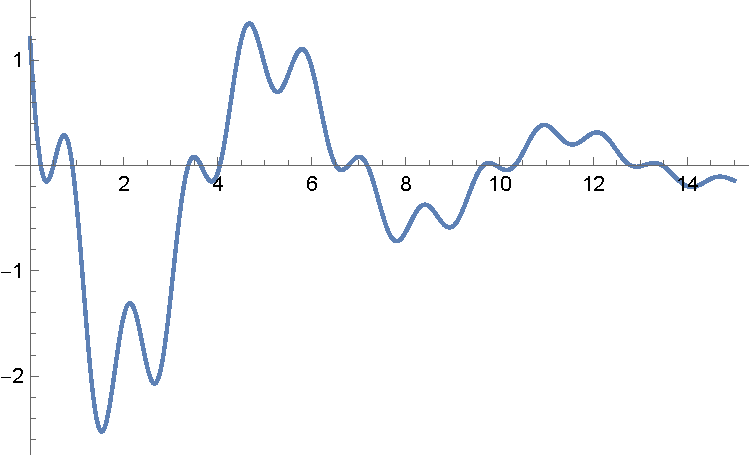
\includegraphics[width=\linewidth]{2dof-b} \caption{}
		\end{subfigure}
		\caption{example of free response in the time domain of the first homogeneous component a 2 degrees of freedom system characterized by poles $p_1 = -0.2 + j$, $p_3 = -0.3 + j5$ and residuals $R_{11} = 3 e^{j1}$ and  $R_{13} = e^{j2}$; in $(a)$ we have the "parts" associated to the poles (in blue $x_{11}$ associated to $p_1$, $x_{13}$ in orange for $p_3$) and in $(b)$ the overall time response $x_{h1}(t) = x_{11}(t) + x_{13}(t)$.  }
	\end{figure}
	
	
\subsubsection{Free vibration and natural frequencies}
	Let's now consider the case where are dumping coefficients $c_i$ are zero, hence the matrix $\mat C$ is identically null. Considering so the homogeneous response assuming as non-zero only $x_{10}$, the previous results simplifies and the rational polynomial has a bi-quadratic denominator (\textbf{RIVEDERE}):
	\[ X_{h1}(s) = \frac{s^3 + s \frac{k_2+ k_3}{m_2}}{ s^4 + \left( \frac{k_2 + k_3}{m_2} + \frac{k_1 + k_2}{m_1} \right) s^2 + \frac{k_1 k_2 + k_2 k_3 + k_3 k_1}{m_1 m_2} } x_{10} \]
	In this case roots are purely imaginary and evaluates to $\pm j \omega_1$ and $\pm j \omega_2$: such values $\omega_i$ are the so called \de{natural frequencies} of the system, meaning that if the system is not subjected to any force, it will vibrate as a linear combination of sinusoidal functions pulsating at such frequencies. Having that the homogeneous response can be regarded as
	\[ X_{hom}(s) = \vec{R_{11} \\ R_{21} } e^{p_1 t} + \vec{R_{12} \\ R_{22} } e^{p_2 t} + \vec{R_{13} \\ R_{23} } e^{p_3 t} + \vec{R_{14} \\ R_{24} } e^{p_4 t} \]
	and so applying the Laplace transform the free response is made by the components
	\begin{align*}
		x_{h1}(t) &= 2 |R_{11}| \cos\big(\omega_1 t + \arg\{R_{11}\}\big) + 2 |R_{13}| \cos\big(\omega_1 t + \arg\{R_{13}\}\big) \\
		x_{h2}(t) &= 2 |R_{21}| \cos\big(\omega_2 t + \arg\{R_{21}\}\big) + 2 |R_{23}| \cos\big(\omega_1 t + \arg\{R_{23}\}\big) 		
	\end{align*}
	In this case where there's no damping, is mathematically proven that the arguments of corresponding residuals $R_{1i}\leftrightarrow R_{2i}$ can only be in phase or in phase opposition. Considering $\arg\{R_{1i}\} = \alpha$ then it means that $\arg\{R_{2i}\}$ can only be $\alpha$ or $\alpha +\pi$. Considering that $\cos(\alpha + \pi) = -\cos\alpha$, we can rewrite the the time response as function of coefficients $u_{ij}$ that now can be negative as
	\begin{equation} \label{eq:2dof:homogeneousresponse}
		 x_{hom} = \underbrace{\vec{u_{11} \\ u_{21}} \cos(\omega_1 t + \alpha)}_\textrm{I mode} + \underbrace{\vec{u_{12} \\ u_{22}} \cos(\omega_2 t + \beta)}_\textrm{II mode}
	\end{equation}
	The underlined terms are the so called \de{natural modes} of vibrations of the system; in general any $n$ degrees of freedom system results in $n$ different natural frequencies with $n$  vectors $\vett u_i \in \mathds R^n$ associated to the modal responses. Such natural modes allows to fully describe the homogeneous response of the systems, in fact any free oscillation is a linear combination of linear modes. Considering in fact the starting systems model
	\[ \mat M \ddvett x + \mat K \vett x= \vett 0 \]
	substituting the first mode of the system (respect to that is shown in equation \ref{eq:2dof:homogeneousresponse}) we determine
	\[ -\omega_1^2 \mat M \vec{u_{11} \\ u_{21}} \cos(\omega_1 t + \alpha)  + \mat K \vec{u_{11} \\ u_{21}} \cos(\omega_1 t + \alpha) = \vett 0  \]
	In order to obtain a true relationship independent on the time $t$ we consider we have to solve the eigenvalue-eigenvector problem of the form
	\[ \Big(\mat K - \omega^2 \mat M\Big) \vett u = \vett 0 \]
	We can in fact compute the characteristic polynomial as function of $\omega^2$ and this determines the natural frequencies $\omega_1, \omega_2$  (having a polynomial in $\omega^2$, each root $\omega_i^2$ of the characteristic polynomial results in two opposite value $\omega_i$ and $-\omega_i$). Determined such parameters we can compute the eigenvectors $\vett u_i = (u_{1i}, u_{2i})$ associated to the system. Such vectors are proven to be orthogonal, in fact considering that they are solution of the system $-\omega_i^2 \mat M \vett u_i + \mat K \vett u_i = \vett 0$, by firstly considering the first mode and premultiplying it by $\vett u_2^T$ results in the scalar
	\[ -\omega_1^2  \vett u_2^t \mat M \vett u_1 + \vett u_2^T \mat K \vett u_1 = 0 \]
	Knowing that a scalar transposed coincides with himself, applying the rules of the transposition of multiplication what we obtain is that
	\[ -\omega_1^2 \vett u_1^T\mat M^T \vett u_2 + \vett u_1^T \mat K^T \vett u_2 = 0 \]
	If we moreover consider that the matrices $\mat M,\mat K$ are mainly symmetric	
	\[ (I) \qquad -\omega_1^2 \vett u_1^T\mat M \vett u_2 + \vett u_1^T \mat K \vett u_2 = 0 \]
	Considering instead now the values obtained using the second mode and premultiplying everything by $\vett u_1^T$ what we get is
	\[ (II) \qquad -\omega_2^2 \vett u_1^T \mat M \vett u_2 + \vett u_1^T \mat K \vett u_2 = 0 \]
	Computing the difference $(II)-(I)$ we obtain
	\[ \big(\omega_2^2-\omega_1^2\big) \vett u_1^T \mat M \vett u_2 + \cancel{\vett u_1^T \mat K \vett u_2 - \vett u_1^T \mat K \vett u_2 } = 0  \]
	We so obtained that the vectors $\vett u_1$ and $\vett u_2$ are representing orthogonal modes respect to the mass matrix $\mat M$, but it happens so also with respect to the stiffness matrix $\mat K$, in fact
	\[ \cancel{-\omega_1^2 \vett u_2^T \mat M \vett y_1} + \vett u_2^T \mat K \vett u_1 = 0 \qquad \Leftrightarrow \qquad \vett u_2^T \mat K \vett u_1 = 0  \]	
	
	Regarding $\cos(\omega_1 t + \alpha)$ as a function $q_1(t)$ and similarly $\cos(\omega_2 t + \beta) = q_2(t)$, then the homogeneous response of the system can be described as a linear combination of orthogonal modes
	\begin{equation}
		\vett x = \vec{x_1 \\ x_2} = \matrix{u_{11} & u_{12} \\ u_{21} & u_{22} } \vec{q_1 \\ q_2} = \mat U \vett q
	\end{equation}
	where $\mat U$ is the \de{modal matrix}.
	
	Considering now the more general case of the dynamical system modelled as $\mat M \ddvett x + \mat K \vett x = \vett f$, if we consider the states $\vett x$ as the linear combination of the modal responses what we obtain is that we have \textit{decoupled} differential equations, in fact
	\begin{align*}
		\mat M (\vett u_1 \ddot q_1 + \vett u_2 \ddot q_2) + \mat K(\vett u_1  q_1 + \vett u_2  q_2)  & = \vett f \\
		\vett u_1^T \mat M \vett u_1 \ddot q_1 + \cancel{\vett  u_1^T \mat M \vett u_2 \ddot q_2} + \vett  u_1^T \mat K \vett u_1  q_1 + \cancel{ \vett  u_1^T \mat K \vett u_2  q_2}  & = \vett u_1^T\vett f \\
		\vett u_1^T \mat M \vett u_1 \ddot q_1 + \omega_1^2 \vett  u_1^T \mat M \vett u_1  q_1  & = \vett u_1^T\vett f
	\end{align*}
	Considering that each product $\vett u_i^T \mat M \vett u_i$ evaluates to a scalar $b_i$ representing the so called \de{modal mass} of the system, but that also $\vett u_i^T \vett f$ evaluates to the \textbf{modal force} $f_i$, we obtain the \textit{compact} formulation
	\[ b_1 \ddot q_1 - \omega_1^2 b_1 q_1 = f_1 \]
		
		
		
		
		
		
		
		